\documentclass[tikz,border=3pt]{standalone}
\usepackage[utf8]{inputenc}
\usepackage[T1]{fontenc}
\usepackage{lmodern}
\renewcommand{\familydefault}{\sfdefault}
\usepackage{sansmath}\sansmath
\usepackage{chemfig}
\usepackage{pgfplots}\pgfplotsset{compat=1.18,/pgf/number format/use comma,/pgf/number format/1000 sep={.}}
\usetikzlibrary{arrows.meta,calc,positioning,decorations.pathmorphing,patterns}
% paleta del sitio
\definecolor{nar}{HTML}{E8680C}\definecolor{narc}{HTML}{FFB35C}\definecolor{hielo}{HTML}{FFF3E8}
\definecolor{tinta}{HTML}{1D1D1F}\definecolor{gris}{HTML}{6E6E73}\definecolor{lila}{HTML}{7C5CF0}
\definecolor{azul}{HTML}{2F6FD6}\definecolor{menta}{HTML}{17A673}\definecolor{coral}{HTML}{E8342A}
\begin{document}
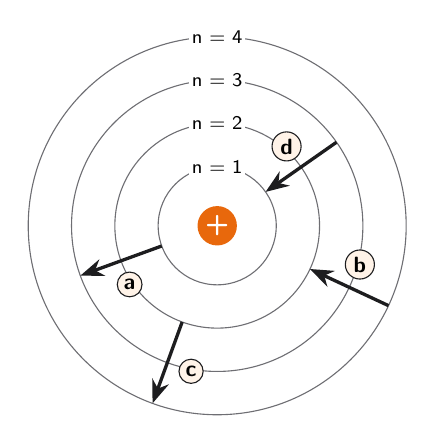
\begin{tikzpicture}[font=\small]
\draw[gris] (0,0) circle (0.75);
\draw[gris] (0,0) circle (1.3);
\draw[gris] (0,0) circle (1.85);
\draw[gris] (0,0) circle (2.4);
\fill[nar] (0,0) circle (0.25); \node[text=white,font=\bfseries] at (0,0) {+};
\node[font=\scriptsize,fill=white,inner sep=1pt] at (0,0.75) {n = 1};
\node[font=\scriptsize,fill=white,inner sep=1pt] at (0,1.3) {n = 2};
\node[font=\scriptsize,fill=white,inner sep=1pt] at (0,1.85) {n = 3};
\node[font=\scriptsize,fill=white,inner sep=1pt] at (0,2.4) {n = 4};
\draw[tinta,very thick,-{Stealth}] (-0.705,-0.257) -- (-1.738,-0.633);
\node[draw=tinta,circle,fill=hielo,inner sep=1.2pt,font=\footnotesize\bfseries] at (-1.112,-0.745) {a};
\draw[tinta,very thick,-{Stealth}] (2.175,-1.014) -- (1.178,-0.549);
\node[draw=tinta,circle,fill=hielo,inner sep=1.2pt,font=\footnotesize\bfseries] at (1.812,-0.492) {b};
\draw[tinta,very thick,-{Stealth}] (-0.445,-1.222) -- (-0.821,-2.255);
\node[draw=tinta,circle,fill=hielo,inner sep=1.2pt,font=\footnotesize\bfseries] at (-0.332,-1.848) {c};
\draw[tinta,very thick,-{Stealth}] (1.515,1.061) -- (0.614,0.43);
\node[draw=tinta,circle,fill=hielo,inner sep=1.2pt,font=\footnotesize\bfseries] at (0.881,1.008) {d};

\end{tikzpicture}
\end{document}
